\documentclass{beamer}
 
\usepackage[utf8]{inputenc}
\usepackage[english]{babel}
\usepackage{amsmath}
\usepackage{amsfonts}
\usepackage{amssymb}
\usepackage{graphicx} 
\usepackage{latexsym} 
\usepackage{listings}
\usepackage{xcolor}
\usepackage{soul}
\usepackage[T1]{fontenc}
\usepackage{amsthm}
\usepackage{mathtools}
\usepackage{setspace}
\usepackage{array,multirow,makecell}
\usepackage{geometry}
\usepackage{textcomp}
\usepackage{float}
\usepackage{bbold}
\usepackage{wrapfig}
\usepackage{textpos}

\rmfamily

\usetheme{Madrid}
%%\usecolortheme{beaver}



\title{LP 36 Diffraction par des structures périodiques}
\author{}
\date{Agregation 2019}

\begin{document}
	
\begin{frame}
\titlepage
\end{frame}

\addtocounter{framenumber}{-1}
\title{Diffraction par des structures périodiques}

\begin{frame}
\frametitle{Réseau de fente idéal}
\centerline{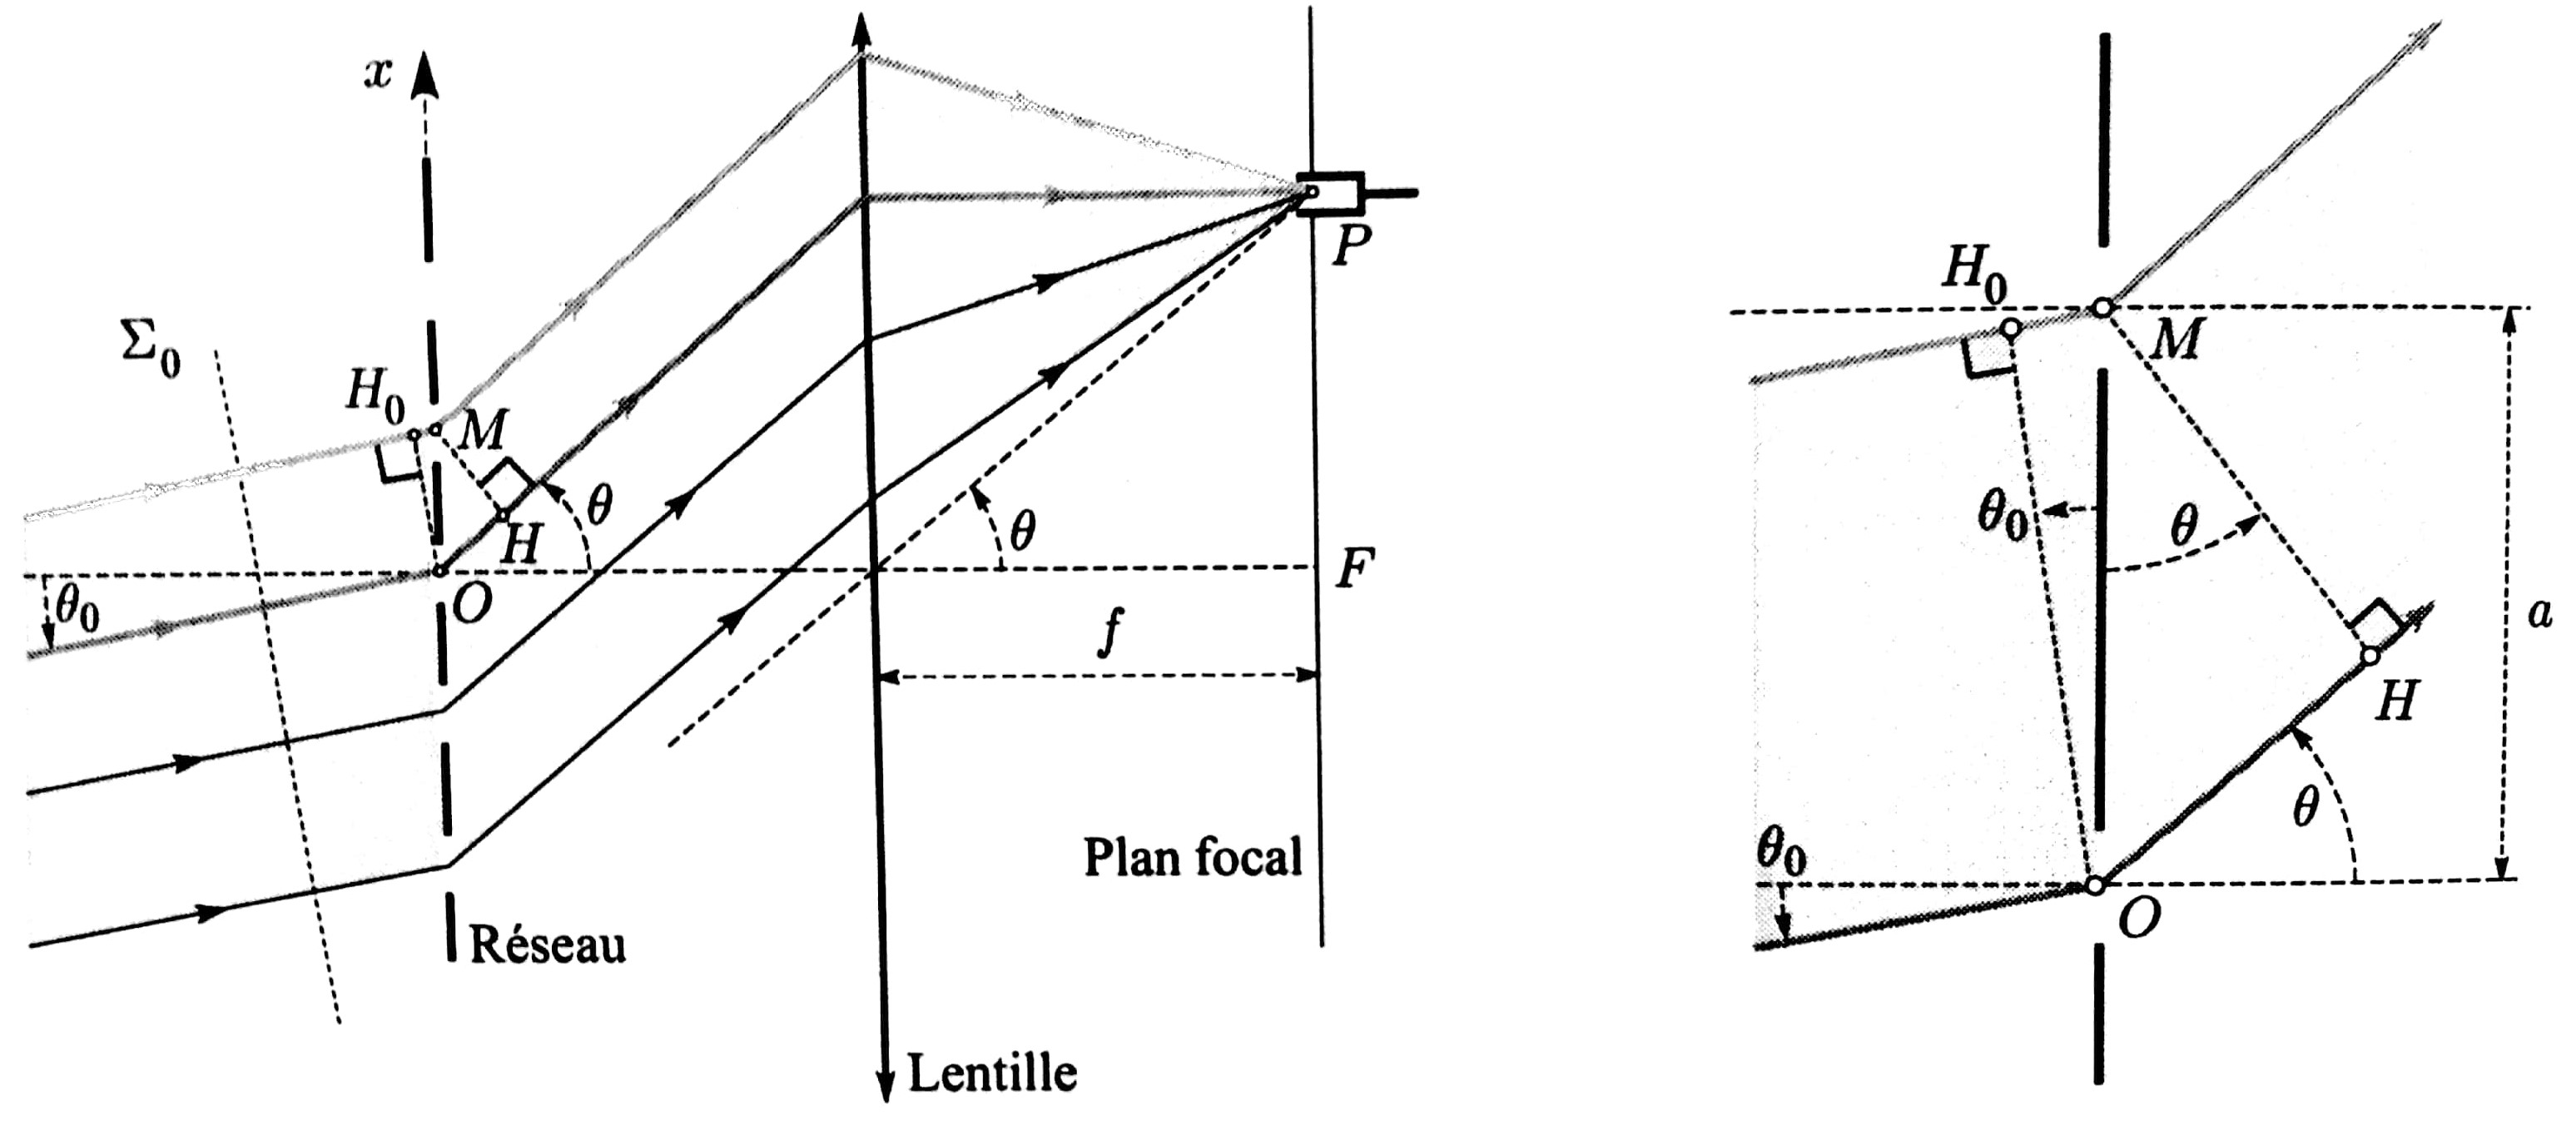
\includegraphics[width=11cm]{reseau}}
\end{frame}

\begin{frame}
\frametitle{Intensité à l'infini dans le cas d'un réseau de fentes}
\centerline{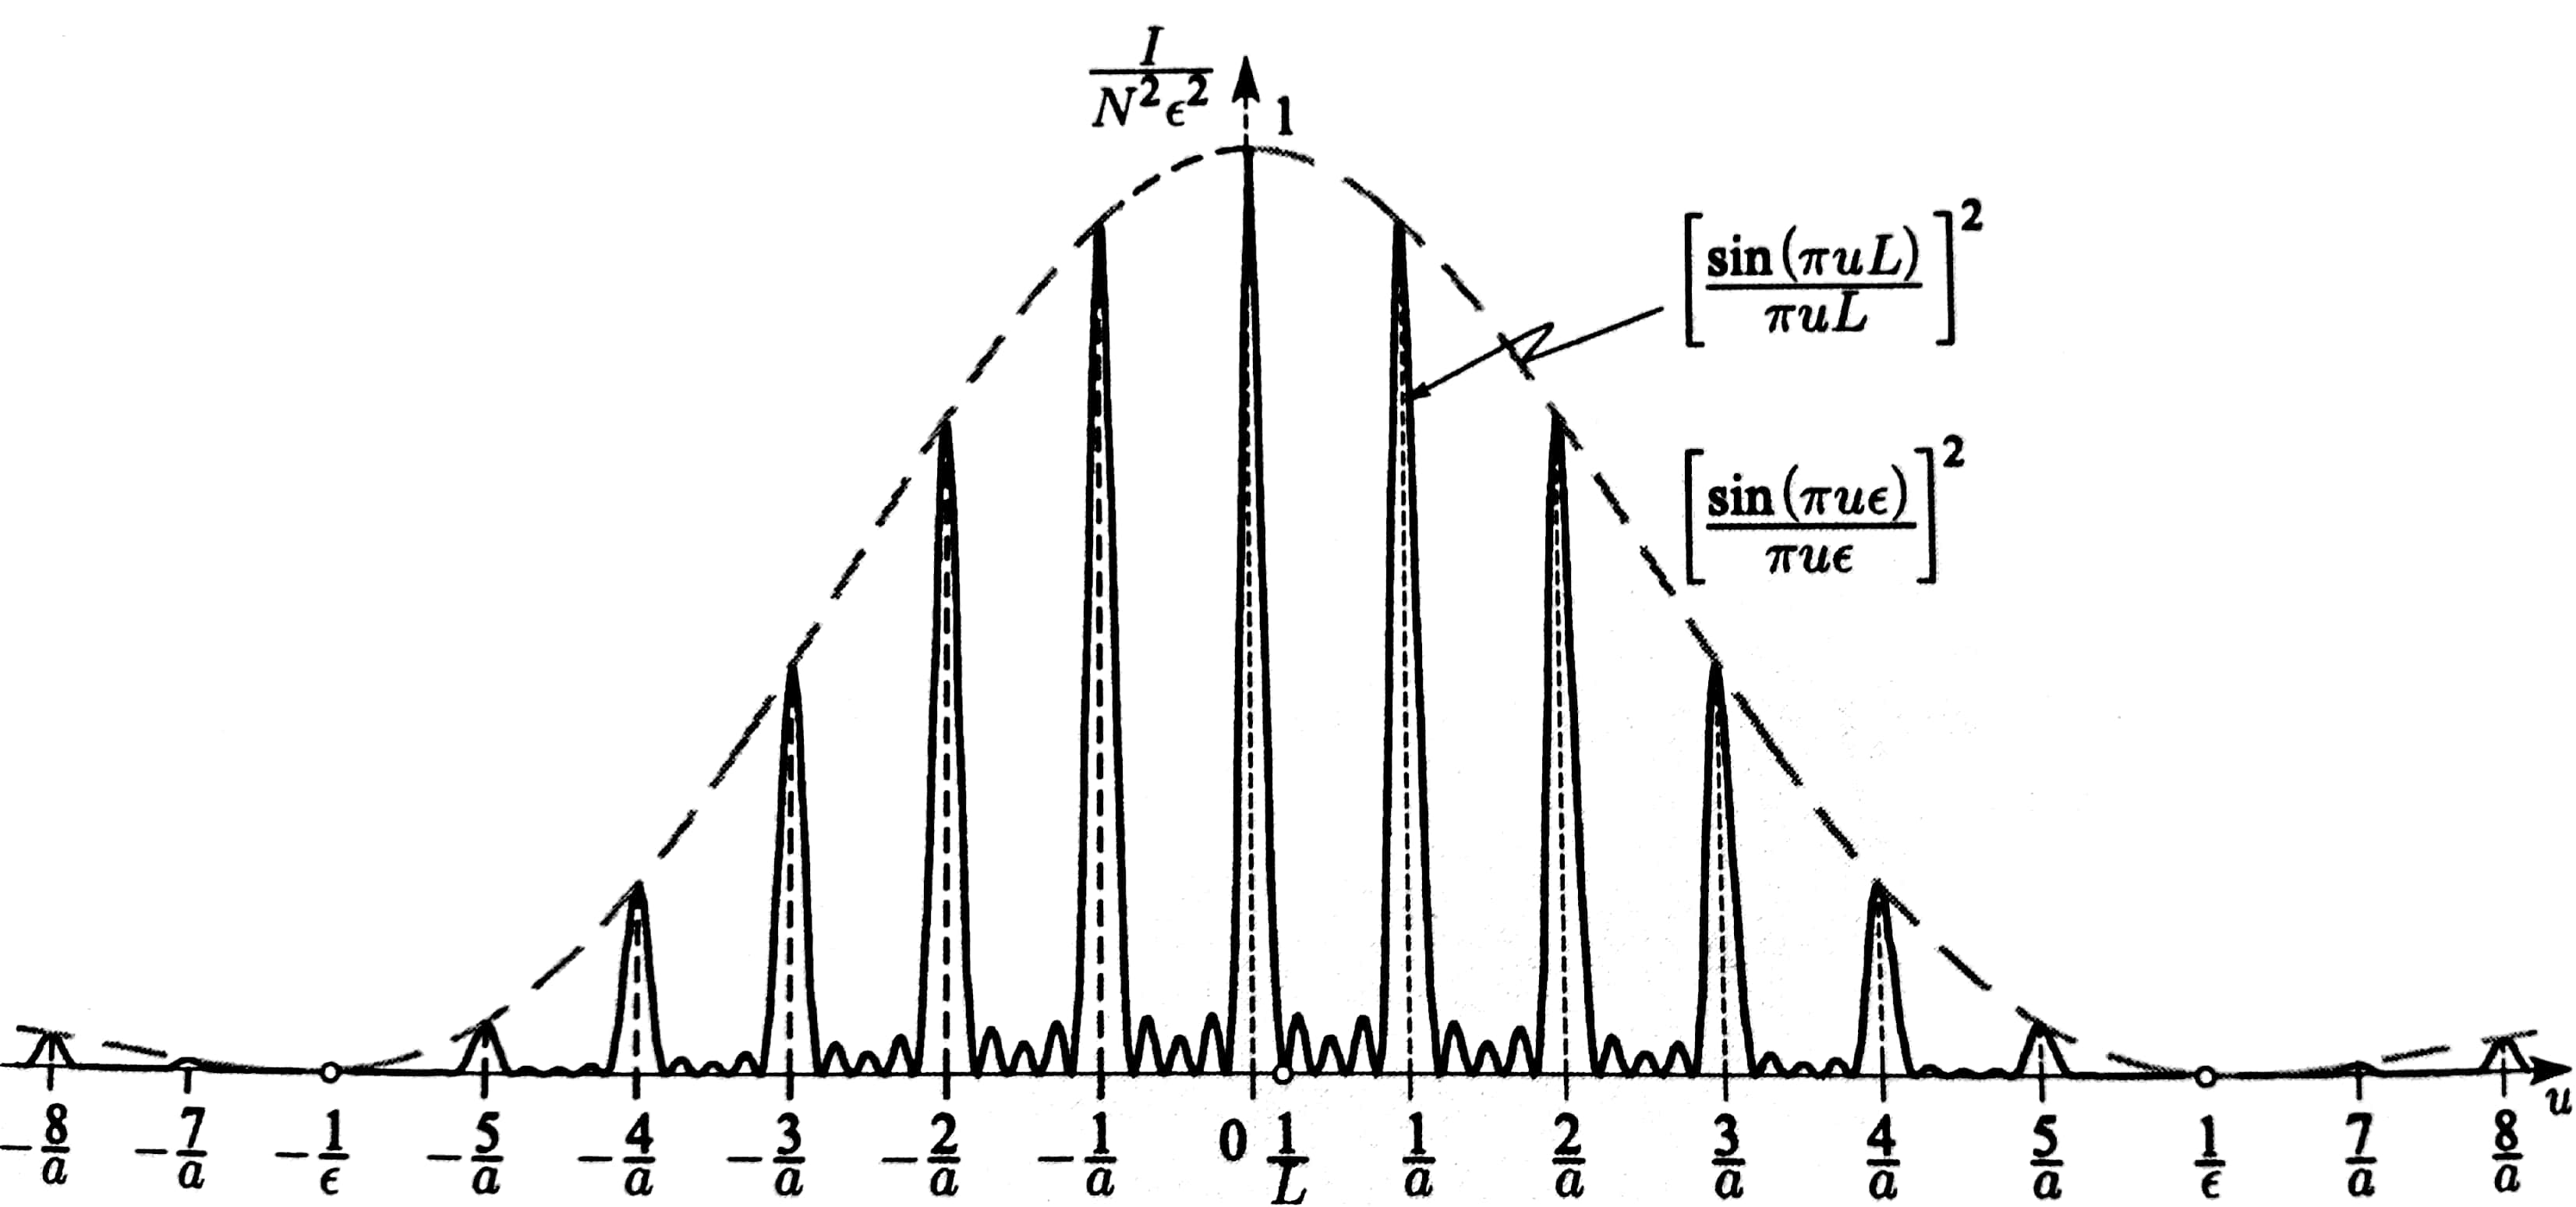
\includegraphics[width=12cm]{intensite}}
\end{frame}


\begin{frame}
\frametitle{Relation de Bragg}
\centerline{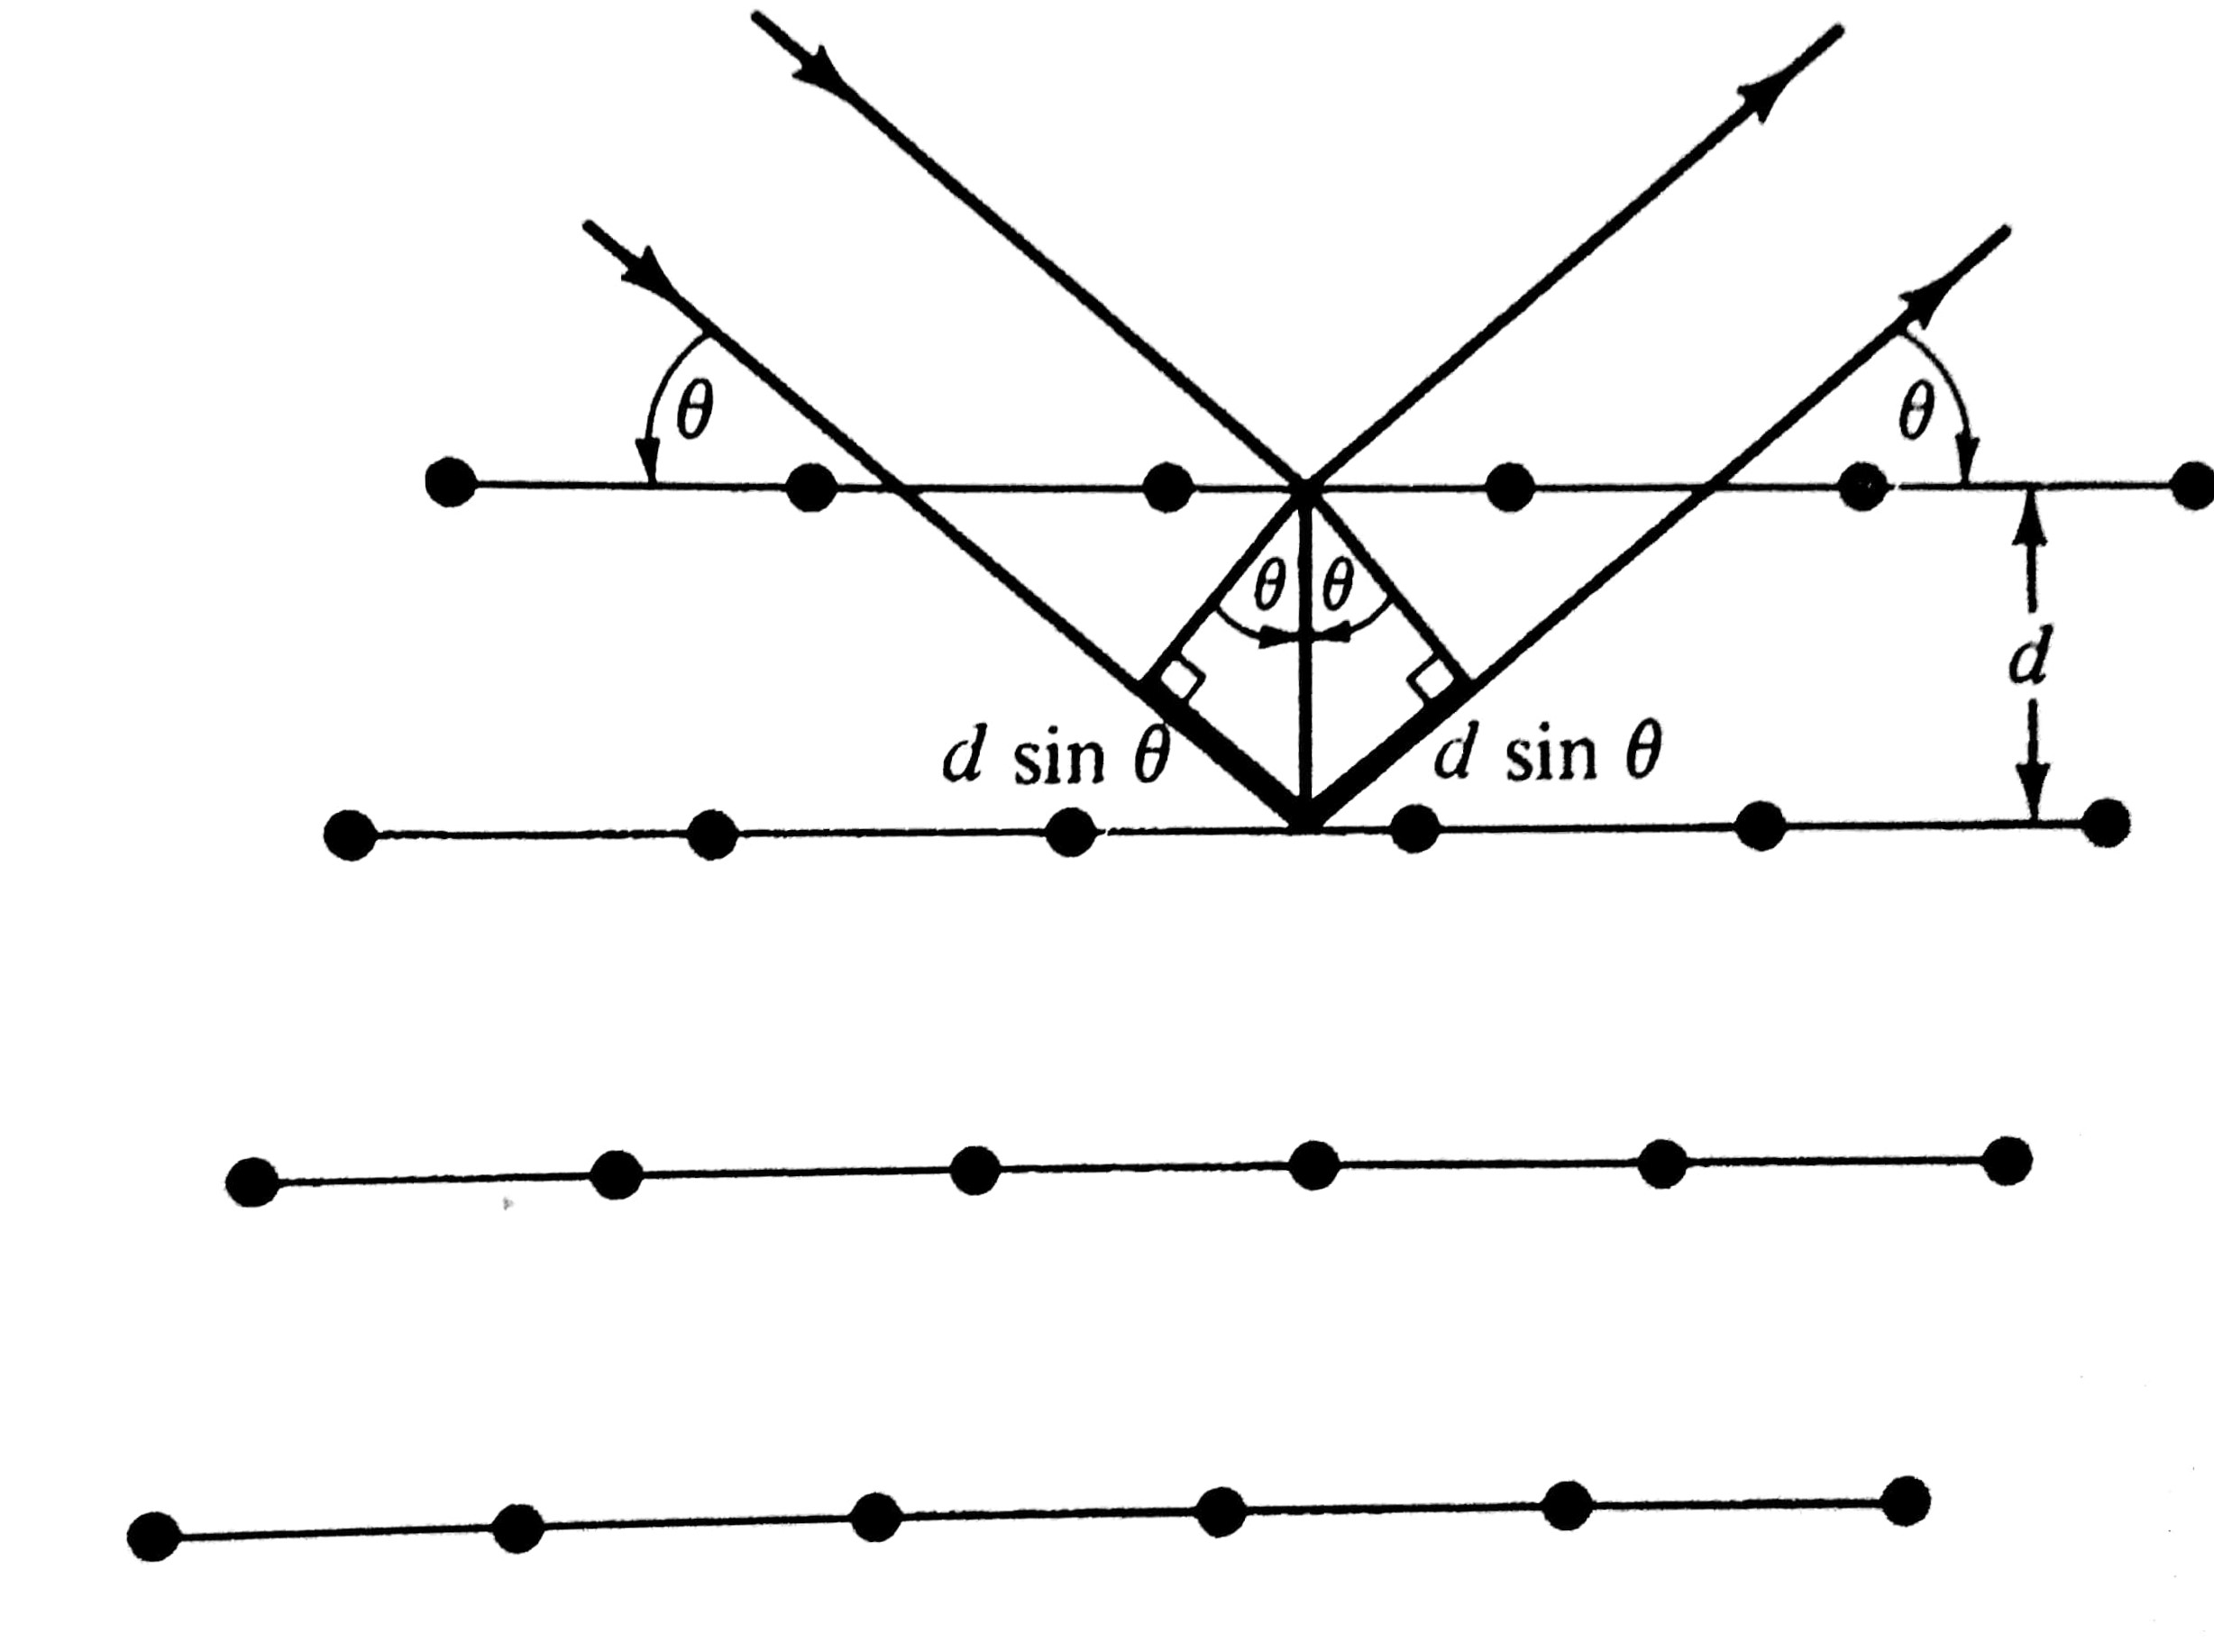
\includegraphics[width=7cm]{bragg}}
\end{frame}


\end{document}